\documentclass[deutsch]{llncs}
\usepackage{multirow, cellspace}
\usepackage{microtype}
\usepackage{tabularx}
\usepackage{ltablex}
\usepackage{amssymb}
\usepackage{amsmath}
\usepackage[utf8]{inputenc} %Umlaute
\usepackage{amssymb}
\usepackage{upgreek}
\usepackage{graphicx}
\usepackage{amsmath}
\usepackage{array}

% subfigure
\usepackage{caption}
\usepackage{subcaption}
%

\usepackage{adjustbox}

\renewcommand{\arraystretch}{1.5}
\renewcommand{\labelenumi}{\Alph{enumi}.}
\setlength{\jot}{10pt}

\begin{document}

\title{Intelligente Sehsysteme - Übungsblatt 4}


\author{Hendrik Walther, Jan Konrad, Berkan Kaya}
\institute{}
\maketitle
\section{ImageToolBox: Gamma-Korrektur}
\begin{enumerate}
	\setcounter{enumi}{1}
	\item Eine Gamma-Korrektur mit $\gamma=3$ dunkelt das Bild ab. \\
	      Der Verlauf der Korrekturfunktion zeigt, dass niedrige Intensitätswerte gestaucht werden: $[0,0.5] \rightarrow [0,0.2]$\\
	      Hohe Intensitätswerte werden gespreizt: $[0.8,1] \rightarrow [0.5,1]$ \\

	      Eine Gamma-Korrektur mit $\gamma=1$ hat keinen Effekt. \\
	      Der Verlauf der Korrekturfunktion zeigt, dass jeder Intensitätswert unverändert bleibt: $T_\gamma(I)=I$ \\

	      Eine Gamma-Korrektur mit $\gamma=0.3$ hellt das Bild auf. \\
	      Der Verlauf der Korrekturfunktion zeigt, dass niedrige Intensitätswerte gespreizt werden: $[0,0.2] \rightarrow [0,0.6]$\\
	      Hohe Intensitätswerte werden gestaucht: $[0.5,1] \rightarrow [0.8,1]$
\end{enumerate}

\begin{figure}
	\centering
	\begin{subfigure}{.32\textwidth}
		\centering
		
\includegraphics[width=.99\linewidth]{A1/gamma=3.png}
		\caption{$\gamma=3$}
	\end{subfigure}
	\begin{subfigure}{.32\textwidth}
		\centering
		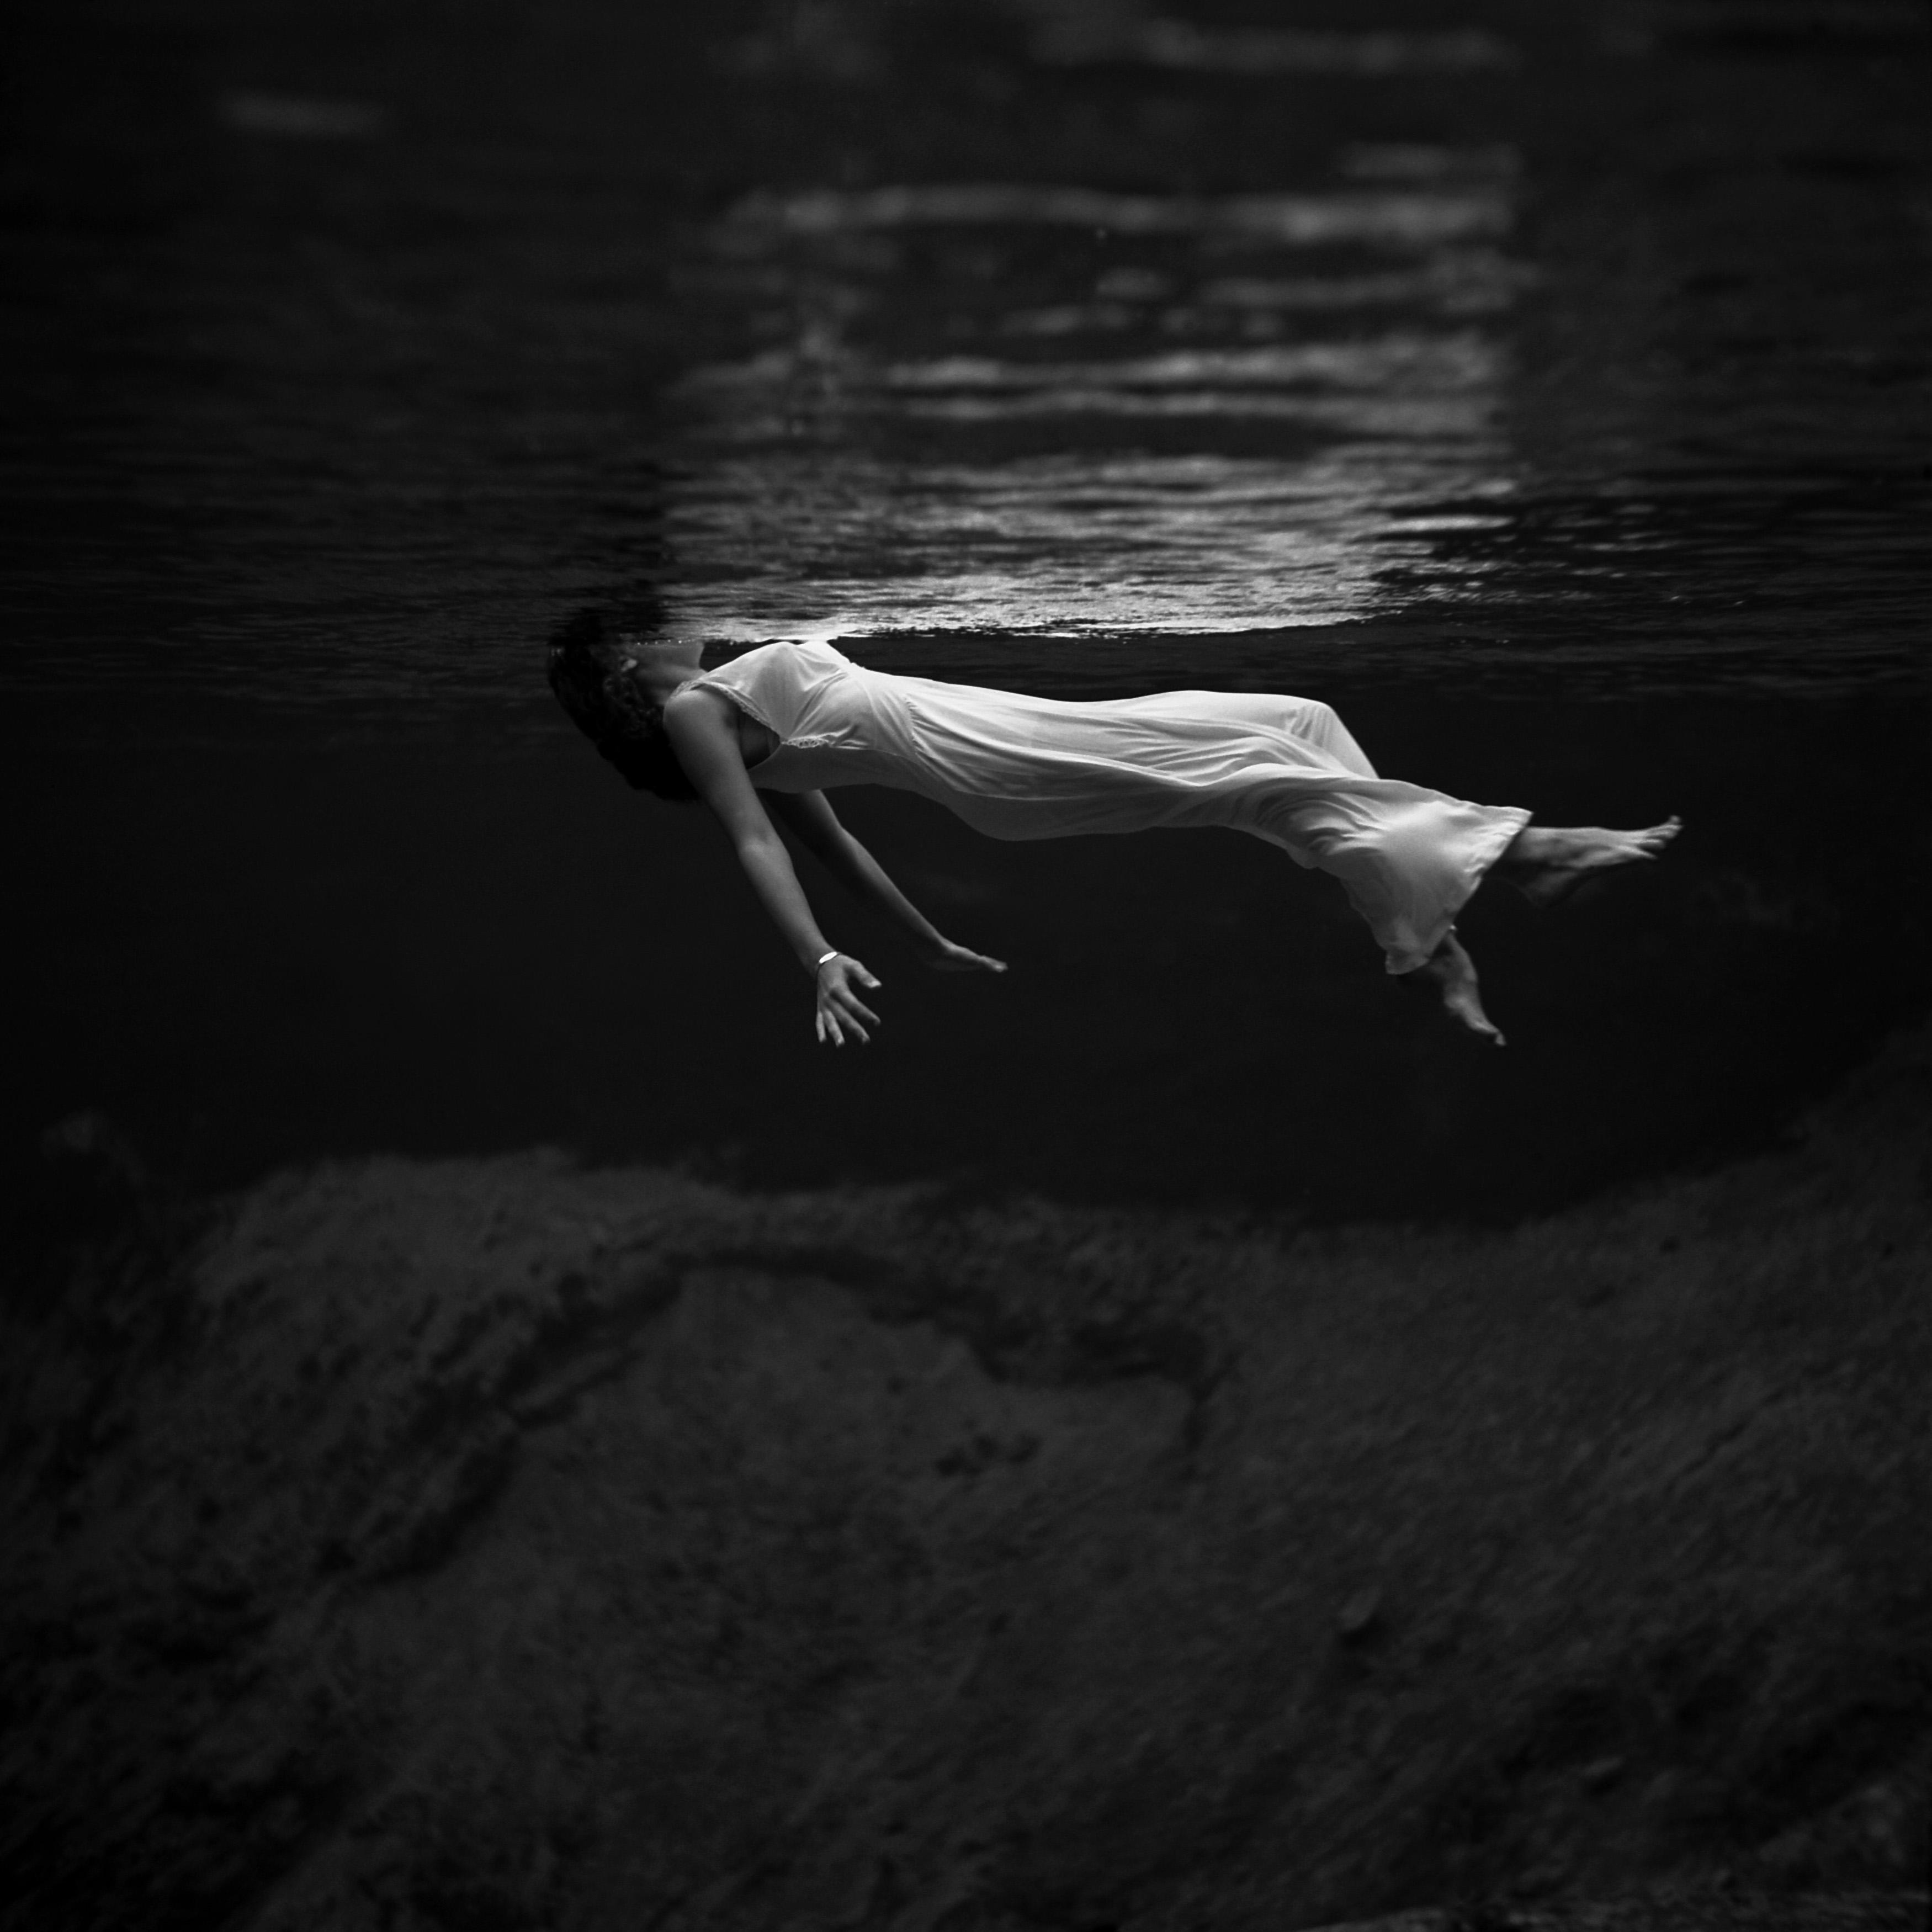
\includegraphics[width=.99\linewidth]{A1/gamma=1.png}
		\caption{$\gamma=1$}
	\end{subfigure}
	\begin{subfigure}{.32\textwidth}
		\centering
		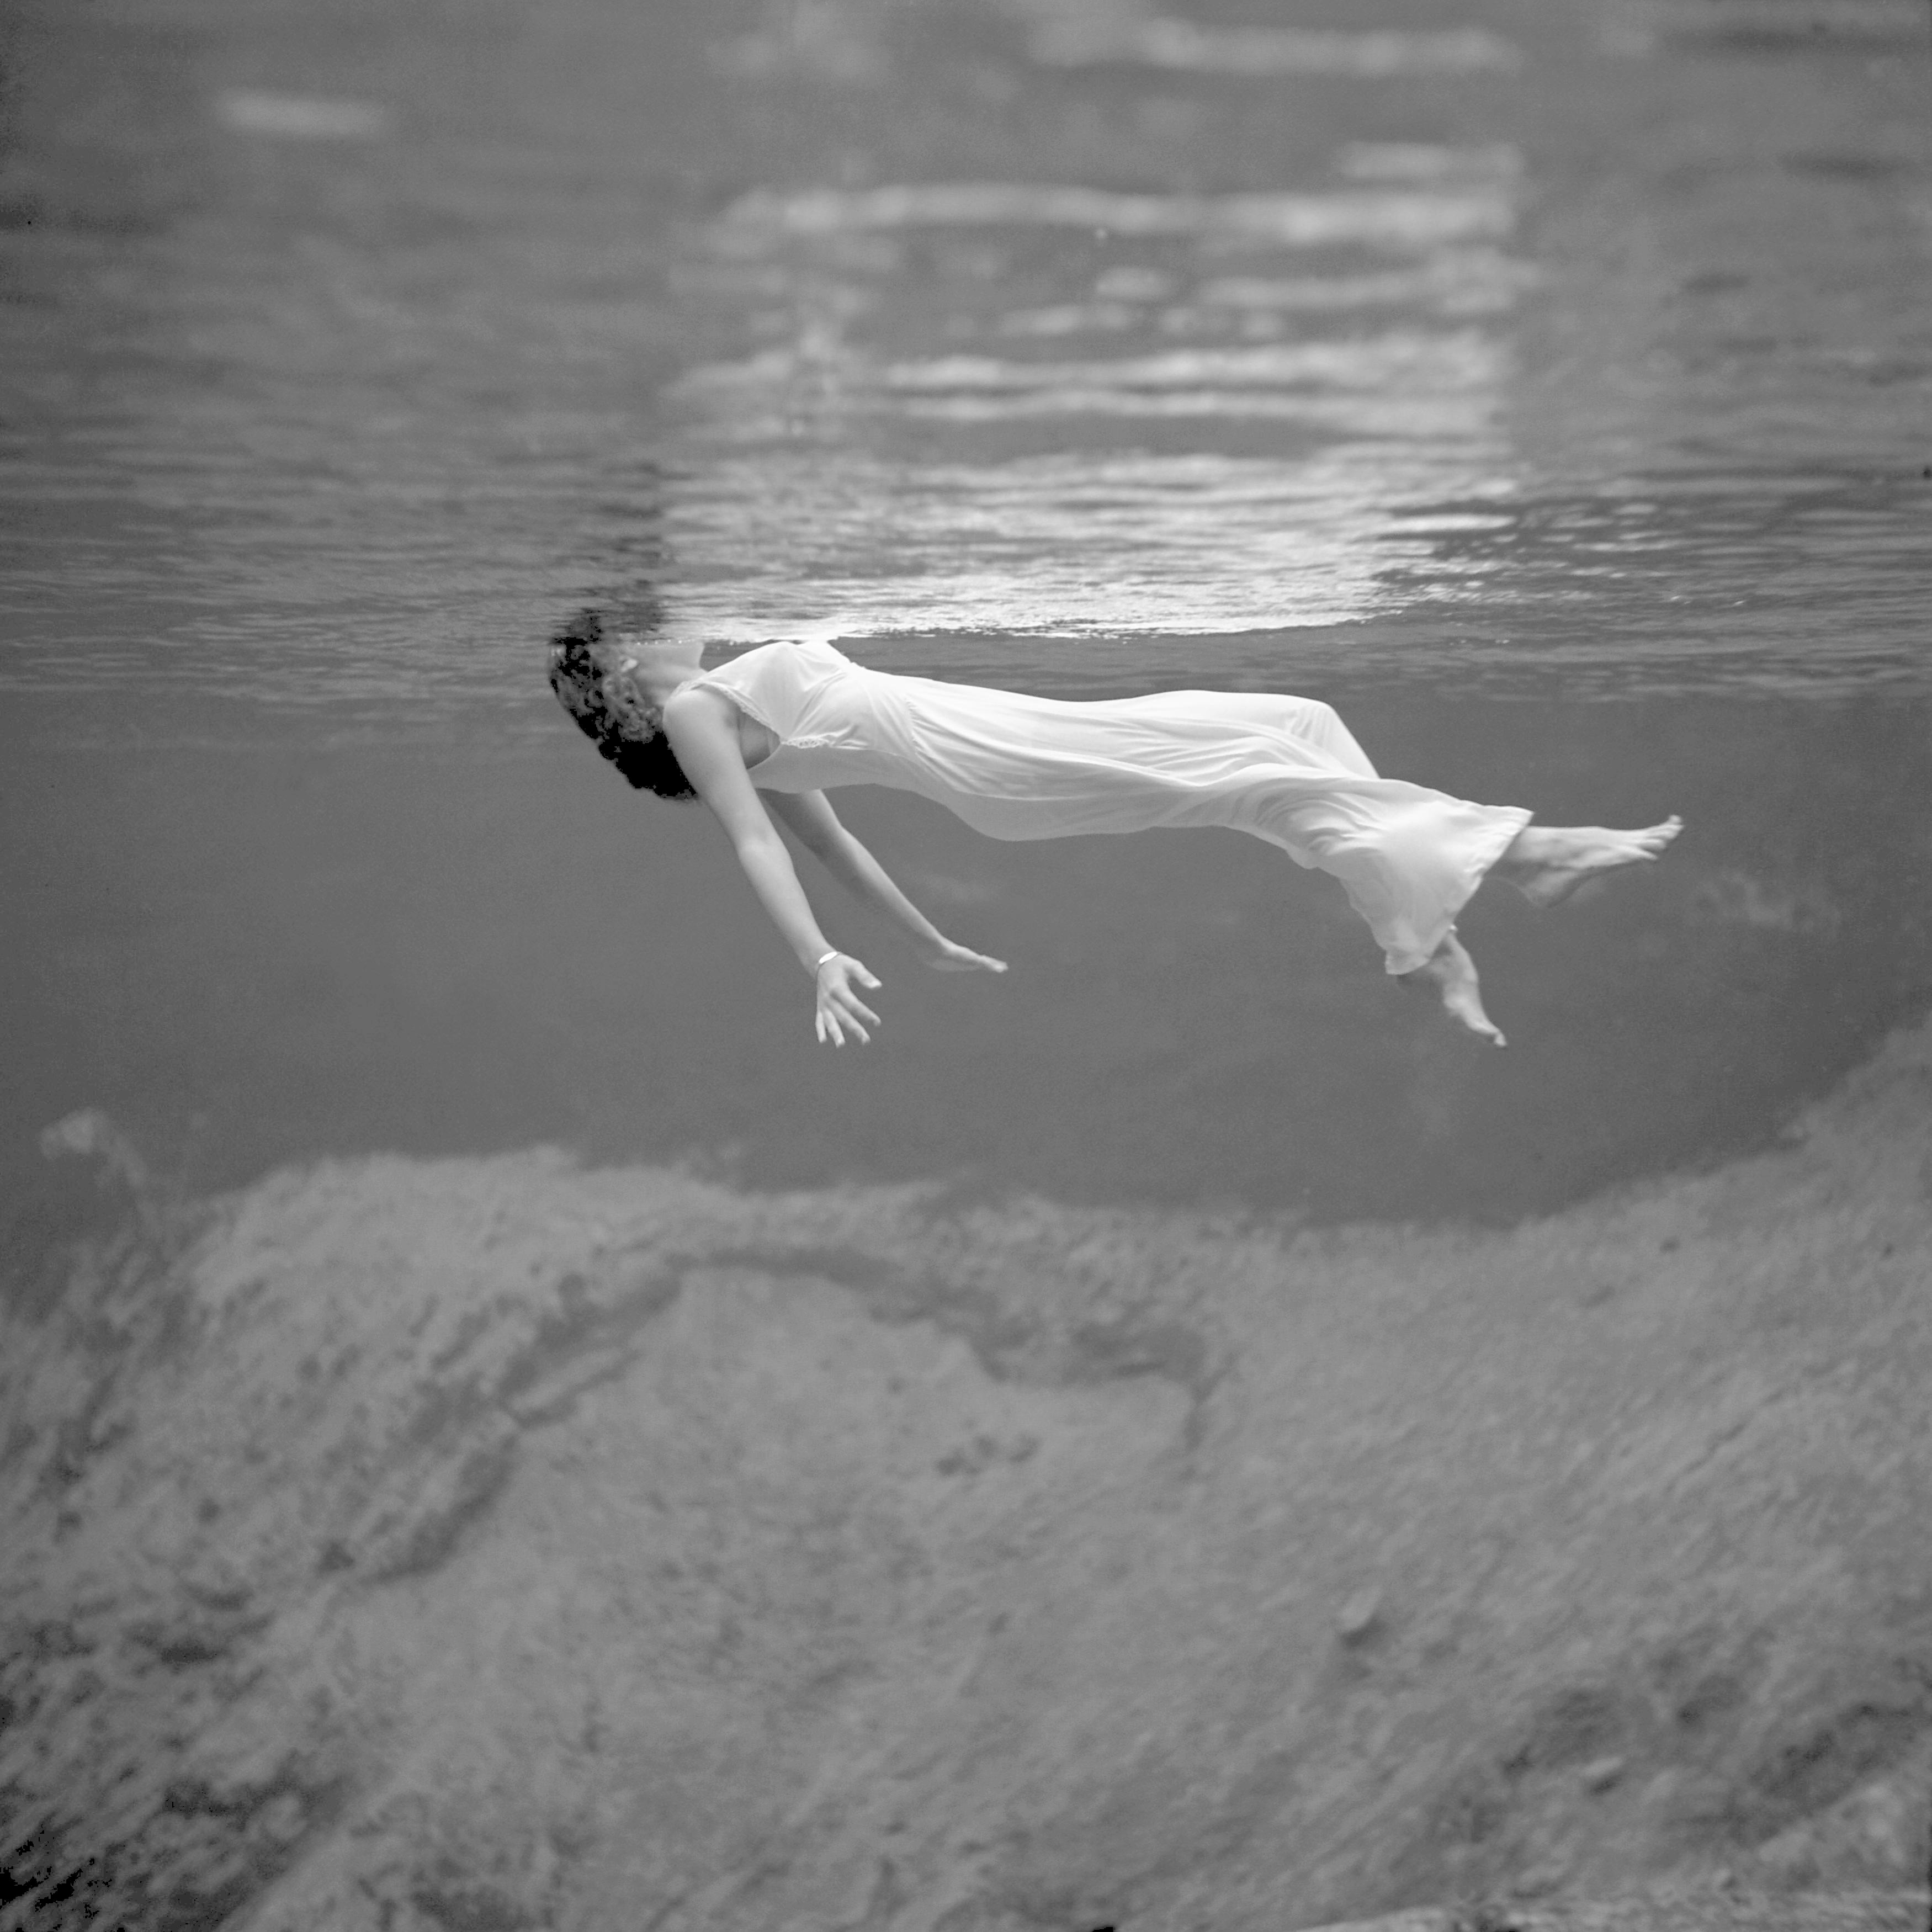
\includegraphics[width=.99\linewidth]{A1/gamma=0.3.png}
		\caption{$\gamma=0.3$}
	\end{subfigure}
\end{figure}
\newpage
\setcounter{section}{2}
\section{ImageToolBox: Diffusionsfilter }

\begin{figure}
	\centering
	\begin{subfigure}{.49\textwidth}
		\centering
		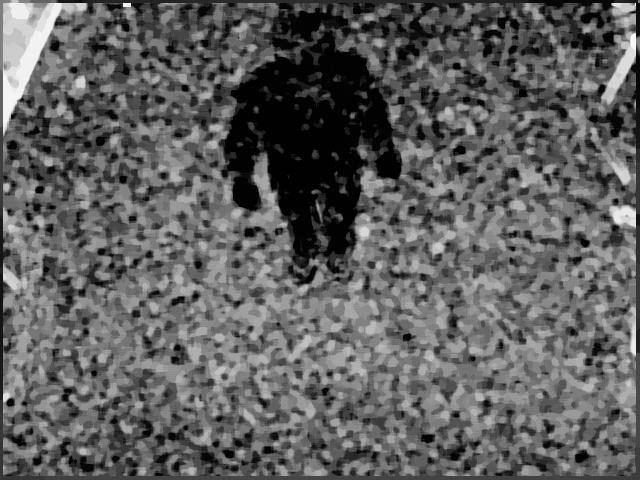
\includegraphics[width=.99\linewidth]{A3/lambda0.5.jpg}
		\caption{$\lambda=0.5$}
	\end{subfigure}
	\begin{subfigure}{.49\textwidth}
		\centering
		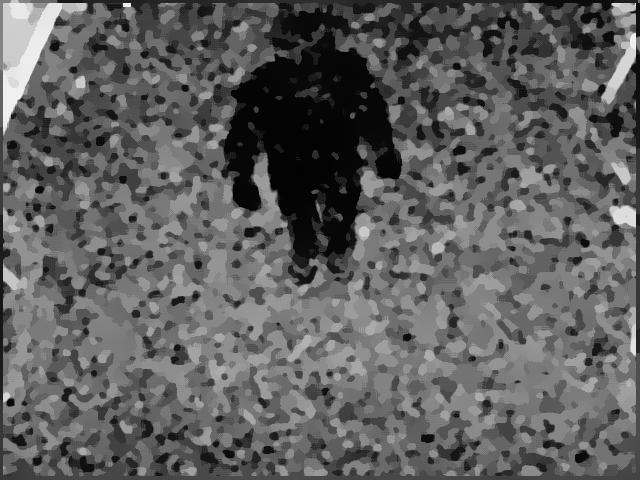
\includegraphics[width=.99\linewidth]{A3/lambda1.jpg}
		\caption{$\lambda=1$}
	\end{subfigure}
	\begin{subfigure}{.49\textwidth}
		\centering
		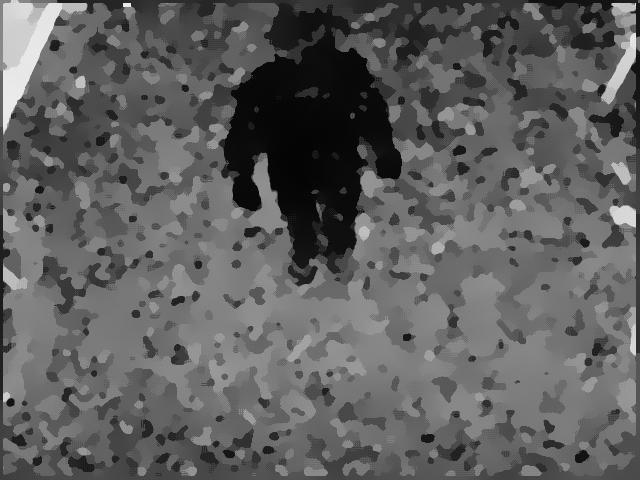
\includegraphics[width=.99\linewidth]{A3/lambda1.5.jpg}
		\caption{$\lambda=1.5$}
	\end{subfigure}
	\begin{subfigure}{.49\textwidth}
		\centering
		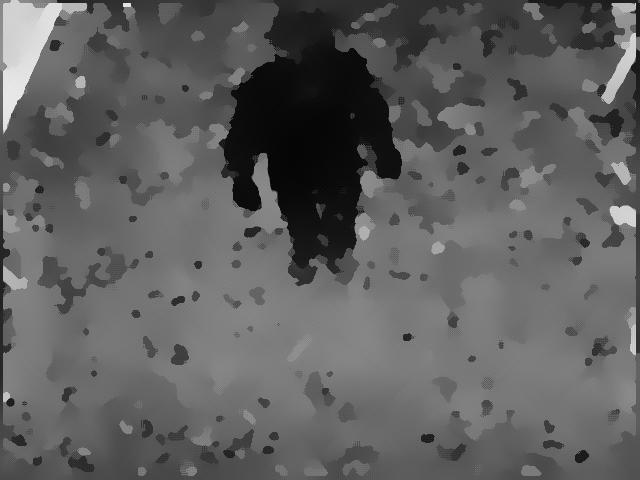
\includegraphics[width=.99\linewidth]{A3/lambda2.jpg}
		\caption{$\lambda=2$}
	\end{subfigure}

	\caption{Isotropes inhomogenes Diffusionsfilter mit $\epsilon_0=1$ und 500 Iterationen}
\end{figure}
\newpage
\section{Tensorberechnung fur anisotropes inhomogenes Diffusionsfilter}
\begin{enumerate}
	\setlength\itemsep{2em}
	\item $\begin{aligned}[t]
			      \begin{pmatrix}
				      e_{1,1} \\
				      e_{1,2}
			      \end{pmatrix} & = \frac{\nabla u}{\| \nabla u \|}                             \\
			      \begin{pmatrix}
				      e_{2,1} \\
				      e_{2,2}
			      \end{pmatrix} & =
			      \begin{pmatrix}
				      e_{1,2} \\
				      -e_{1,1}
			      \end{pmatrix}                                                                \\
			      \lambda_1       & = \epsilon_0 \frac{\lambda^2}{\| \nabla u \|^2 + \lambda^2} \\
			      \lambda_2       & = 1                                                         \\
			      \nabla u (x,y)  & \approx \begin{pmatrix}
				                                I(x+1,y)-I(x-1,y) \\
				                                I(x,y+1)-I(x,y-1)
			                                \end{pmatrix}
		      \end{aligned}$\\

	      Für $ x,y =3 $ gilt:\\
	      $\begin{aligned}
			      \nabla u (3,3)      & \approx \begin{pmatrix}
				                                    I(4,3)-I(2,3) \\
				                                    I(3,4)-I(3,2)
			                                    \end{pmatrix}
			      = \begin{pmatrix}
				        10 \\
				        10
			        \end{pmatrix}                                                                               \\
			      \| \nabla u(3,3) \| & =\sqrt{10^2+10^2}=10\sqrt{2}                                             \\
			      \begin{pmatrix}
				      e_{1,1} \\
				      e_{1,2}
			      \end{pmatrix}     & = \frac{1}{10\sqrt{2}}  \begin{pmatrix}
				                                                  10 \\
				                                                  10
			                                                  \end{pmatrix} = \frac{1}{\sqrt{2}}  \begin{pmatrix}
				                                                                                      1 \\
				                                                                                      1
			                                                                                      \end{pmatrix} \\
			      \begin{pmatrix}
				      e_{2,1} \\
				      e_{2,2}
			      \end{pmatrix}     & =
			      \frac{1}{\sqrt{2}}  \begin{pmatrix}
				                          1 \\
				                          -1
			                          \end{pmatrix}                                                             \\
			      \lambda_1           & = \epsilon_0 \frac{\lambda^2}{200 + \lambda^2}                           \\
			                          & \text{mit } \epsilon_0=\lambda=1                                         \\
			      \lambda_1           & = \frac{1}{201}                                                          \\
			      \lambda_2           & = 1
		      \end{aligned}$\\
	      \newpage
	\item  $\begin{aligned}[t]
			      \mathbf{D} & =
			      \begin{pmatrix}
				      e_{1,1} & e_{2,1} \\
				      e_{1,2} & e_{2,2}
			      \end{pmatrix}
			      \begin{pmatrix}
				      \lambda_1 & 0         \\
				      0         & \lambda_2
			      \end{pmatrix}
			      \begin{pmatrix}
				      e_{1,1} & e_{1,2} \\
				      e_{2,1} & e_{2,2}
			      \end{pmatrix}                             \\
			                 & =
			      \left(
			      \frac{1}{\sqrt{2}}
			      \begin{pmatrix}
				      1 & 1  \\
				      1 & -1
			      \end{pmatrix}
			      \right)
			      \begin{pmatrix}
				      \frac{1}{201} & 0 \\
				      0             & 1
			      \end{pmatrix}
			      \left(
			      \frac{1}{\sqrt{2}}
			      \begin{pmatrix}
				      1 & 1  \\
				      1 & -1
			      \end{pmatrix}
			      \right)                                       \\
			                 & =
			      \left(
			      \frac{1}{\sqrt{2}}
			      \begin{pmatrix}
				      1 & 1  \\
				      1 & -1
			      \end{pmatrix}
			      \right)
			      \left(
			      \frac{1}{\sqrt{2}}
			      \begin{pmatrix}
				      \frac{1}{201} & 0  \\
				      0             & -1
			      \end{pmatrix}
			      \right)
			      \\
			                 & =    \begin{pmatrix}
				                        \frac{1}{402} & 0           \\
				                        0             & \frac{1}{2}
			                        \end{pmatrix}
		      \end{aligned}$

	\item $ \mathbf{D}$ ist positiv definit, da für alle Eigenvektoren $\lambda_1, \lambda_2 > 0$ gilt.
\end{enumerate}

\end{document}
